% move all configuration stuff into includes file so we can focus on the content
\documentclass[aspectratio=169,hyperref={pdfpagelabels=false,colorlinks=true,linkcolor=white,urlcolor=blue},t]{beamer}

%%%%%%%%%%%%%%%%%%%%%%%%%%%%%%%%%%%%%%%%%%%%%%%%%%%%%%%%%%%%%%%%%%%%%%%%%%%%%%%%%%
%%%%%%%%%%%%%%%%%%%%%%%%%%%%%%%%%%%%%%%%%%%%%%%%%%%%%%%%%%%%%%%%%%%%%%%%%%%%%%%%%%
% packages
\usepackage{pict2e}
\usepackage{epic}
\usepackage{amsmath,amsfonts,amssymb}
\usepackage{units}
\usepackage{fancybox}
\usepackage[absolute,overlay]{textpos} 
\usepackage{media9} % avi2flv: "C:\Program Files\ffmpeg\bin\ffmpeg.exe" -i TuneFreqFilterbank.avi -b 600k -s 441x324 -r 15 -acodec copy TuneFreqFilterbank.flv
\usepackage{animate}
\usepackage{gensymb}
\usepackage{multirow}
\usepackage{silence}
\usepackage[backend=bibtex,style=ieee]{biblatex}
\AtEveryCitekey{\iffootnote{\tiny}{}}
\addbibresource{references}

%%%%%%%%%%%%%%%%%%%%%%%%%%%%%%%%%%%%%%%%%%%%%%%%%%%%%%%%%%%%%%%%%%%%%%%%%%%%%%%%%%
%%%%%%%%%%%%%%%%%%%%%%%%%%%%%%%%%%%%%%%%%%%%%%%%%%%%%%%%%%%%%%%%%%%%%%%%%%%%%%%%%%
% relative paths
\graphicspath{{graph/}}


%%%%%%%%%%%%%%%%%%%%%%%%%%%%%%%%%%%%%%%%%%%%%%%%%%%%%%%%%%%%%%%%%%%%%%%%%%%%%%%%%%
%%%%%%%%%%%%%%%%%%%%%%%%%%%%%%%%%%%%%%%%%%%%%%%%%%%%%%%%%%%%%%%%%%%%%%%%%%%%%%%%%%
% units
\setlength{\unitlength}{1mm}

%%%%%%%%%%%%%%%%%%%%%%%%%%%%%%%%%%%%%%%%%%%%%%%%%%%%%%%%%%%%%%%%%%%%%%%%%%%%%%%%%%
%%%%%%%%%%%%%%%%%%%%%%%%%%%%%%%%%%%%%%%%%%%%%%%%%%%%%%%%%%%%%%%%%%%%%%%%%%%%%%%%%%
% theme & layout
\usetheme{Frankfurt}
\beamertemplatenavigationsymbolsempty
%\setbeamertemplate{frametitle}[smoothbars theme]
\setbeamertemplate{frametitle}
{
    \begin{beamercolorbox}[ht=1.8em,wd=\paperwidth]{frametitle}
        \vspace{-.1em}%
        \hspace{.2em}{\strut\insertframetitle\strut}
        
        \hspace{.2em}\small\strut\insertframesubtitle\strut
        %\hfill
        %
\includegraphics[height=.8cm,keepaspectratio]{CenterMusicTechnology-solid-2lines-white-CoAtag}
        
    \end{beamercolorbox}
    \begin{textblock*}{100mm}(11.6cm,.7cm)
        \includegraphics[height=.8cm,keepaspectratio]{logo_GTCMT_black}
    \end{textblock*}
}

% set this to ensure bulletpoints without subsections
\usepackage{remreset}
\makeatletter
\@removefromreset{subsection}{section}
\makeatother
\setcounter{subsection}{1}

%---------------------------------------------------------------------------------
% appearance
\setbeamercolor{structure}{fg=gtgold}
\setbeamercovered{transparent} %invisible
\setbeamercolor{bibliography entry author}{fg=black}
\setbeamercolor*{bibliography entry title}{fg=black}
\setbeamercolor*{bibliography entry note}{fg=black}

%\usepackage{pgfpages}
%\setbeameroption{show notes}
%\setbeameroption{show notes on second screen=right}
%---------------------------------------------------------------------------------
% fontsize
\let\Tiny=\tiny

%%%%%%%%%%%%%%%%%%%%%%%%%%%%%%%%%%%%%%%%%%%%%%%%%%%%%%%%%%%%%%%%%%%%%%%%%%%%%%%%%%
%%%%%%%%%%%%%%%%%%%%%%%%%%%%%%%%%%%%%%%%%%%%%%%%%%%%%%%%%%%%%%%%%%%%%%%%%%%%%%%%%%
% warnings
\pdfsuppresswarningpagegroup=1
\WarningFilter{biblatex}{Patching footnotes failed}
\WarningFilter{latexfont}{Font shape}
\WarningFilter{latexfont}{Some font shapes}
\WarningFilter{gensymb}{Not defining}


%%%%%%%%%%%%%%%%%%%%%%%%%%%%%%%%%%%%%%%%%%%%%%%%%%%%%%%%%%%%%%%%%%%%%%%%%%%%%%%%%%
%%%%%%%%%%%%%%%%%%%%%%%%%%%%%%%%%%%%%%%%%%%%%%%%%%%%%%%%%%%%%%%%%%%%%%%%%%%%%%%%%%
% title information
\title[]{Introduction to Audio Content Analysis}   
\author[alexander lerch]{alexander lerch} 
%\institute{~}
%\date[Alexander Lerch]{}
\titlegraphic{\vspace{-16mm}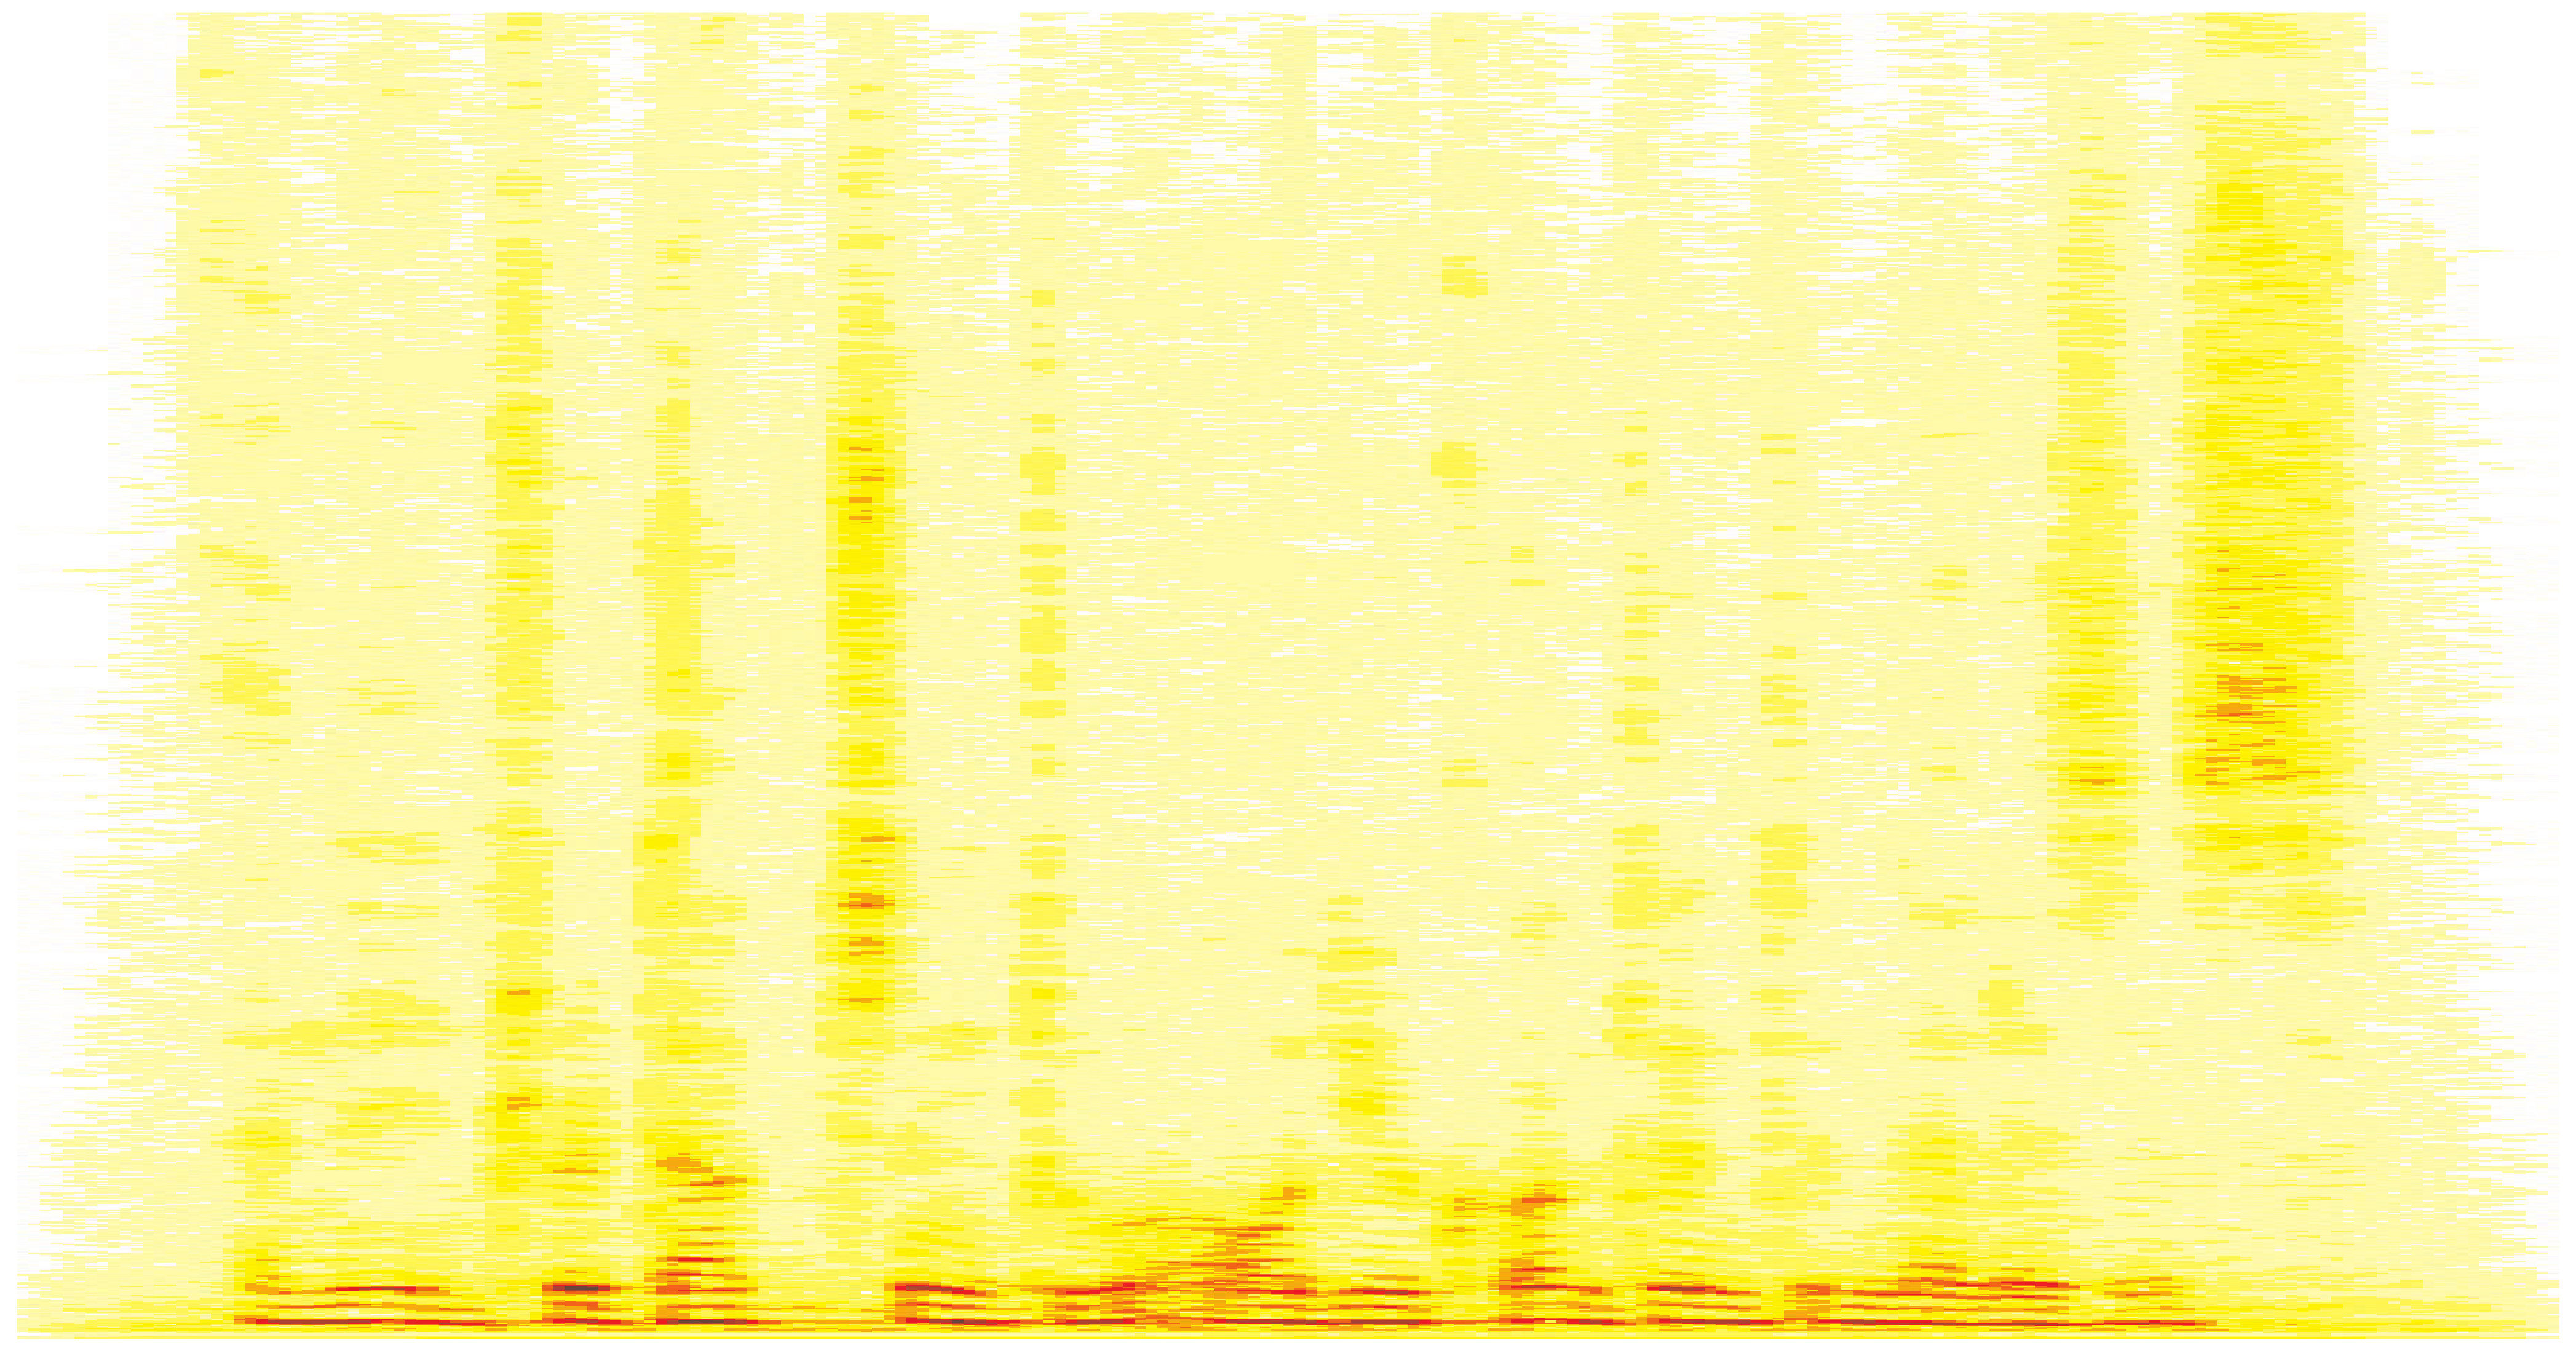
\includegraphics[width=\textwidth,height=3cm]{title}}

%%%%%%%%%%%%%%%%%%%%%%%%%%%%%%%%%%%%%%%%%%%%%%%%%%%%%%%%%%%%%%%%%%%%%%%%%%%%%%%%%%
%%%%%%%%%%%%%%%%%%%%%%%%%%%%%%%%%%%%%%%%%%%%%%%%%%%%%%%%%%%%%%%%%%%%%%%%%%%%%%%%%%
% colors
\definecolor{gtgold}{HTML}{E0AA0F} %{rgb}{0.88,0.66,1,0.06} [234, 170, 0]/256

%%%%%%%%%%%%%%%%%%%%%%%%%%%%%%%%%%%%%%%%%%%%%%%%%%%%%%%%%%%%%%%%%%%%%%%%%%%%%%%%%%
%%%%%%%%%%%%%%%%%%%%%%%%%%%%%%%%%%%%%%%%%%%%%%%%%%%%%%%%%%%%%%%%%%%%%%%%%%%%%%%%%%
% math
\DeclareMathOperator*{\argmax}{argmax}
\DeclareMathOperator*{\argmin}{argmin}
\DeclareMathOperator*{\atan}{atan}
\DeclareMathOperator*{\arcsinh}{arcsinh}
\DeclareMathOperator*{\sign}{sign}
\DeclareMathOperator*{\tcdf}{tcdf}
\DeclareMathOperator*{\si}{sinc}
\DeclareMathOperator*{\princarg}{princarg}
\DeclareMathOperator*{\arccosh}{arccosh}
\DeclareMathOperator*{\hwr}{HWR}
\DeclareMathOperator*{\flip}{flip}
\DeclareMathOperator*{\sinc}{sinc}
\DeclareMathOperator*{\floor}{floor}
\newcommand{\e}{{e}}
\newcommand{\jom}{\mathrm{j}\omega}
\newcommand{\jOm}{\mathrm{j}\Omega}
\newcommand   {\mat}[1]    		{\boldsymbol{\uppercase{#1}}}		%bold
\renewcommand {\vec}[1]    		{\boldsymbol{\lowercase{#1}}}		%bold

%%%%%%%%%%%%%%%%%%%%%%%%%%%%%%%%%%%%%%%%%%%%%%%%%%%%%%%%%%%%%%%%%%%%%%%%%%%%%%%%%%
%%%%%%%%%%%%%%%%%%%%%%%%%%%%%%%%%%%%%%%%%%%%%%%%%%%%%%%%%%%%%%%%%%%%%%%%%%%%%%%%%%
% media9
\newcommand{\includeaudio}[1]{{\includemedia[
                        addresource=audio/#1.mp3,
                        width=5mm,
                        height=5mm,
                        activate=onclick,
                        flashvars={
                            source=audio/#1.mp3  
                            &autoPlay=true
                        }]
                        {
\includegraphics[width=5mm, height=5mm]{SpeakerIcon}}
                        {APlayer.swf}}}
\newcommand{\audioautoplay}[1]{{\begin{center}\includemedia[
                            addresource=audio/#1.mp3,
                            width=.1\linewidth,
                            height=.01\linewidth,
                            activate=pageopen,
                            flashvars={
                                source=audio/#1.mp3  
                                &autoPlay=true
                            }]
                            {}
                            {APlayer.swf}\end{center}}}

\newcommand{\includevideo}[1]{{\begin{center}\includemedia[
                        addresource=video/#1.mp4,
                        width=0.8\linewidth,
                        height=0.4\linewidth,
                        activate=onclick,
                        flashvars={
                            source=video/#1.mp4  
                            &autoPlay=true
                        }]
                        {}
                        {VPlayer.swf}\end{center}}}
\newcommand{\videowithmatlab}[1]{{\begin{center}\includemedia[
                        addresource=video/animate#1.mp4,
                        width=0.8\linewidth,
                        height=0.4\linewidth,
                        activate=onclick,
                        flashvars={
                            source=video/animate#1.mp4  
                            &autoPlay=true
                        }]
                        {}
                        {VPlayer.swf}\end{center}\addreference{matlab source: matlab/animate#1.m}}}
                        

%%%%%%%%%%%%%%%%%%%%%%%%%%%%%%%%%%%%%%%%%%%%%%%%%%%%%%%%%%%%%%%%%%%%%%%%%%%%%%%%%%
%%%%%%%%%%%%%%%%%%%%%%%%%%%%%%%%%%%%%%%%%%%%%%%%%%%%%%%%%%%%%%%%%%%%%%%%%%%%%%%%%%
% other commands
\newcommand{\question}[1]{%\vspace{-4mm}
                          \setbeamercovered{invisible}
                          \begin{columns}[T]
                            \column{.8\textwidth}
                                \textbf{#1}
                            \column{.2\textwidth}
                                \vspace{-8mm}
                                \begin{flushright}
                                     
\includegraphics[scale=.5]{question_mark}
                                \end{flushright}
                                \vspace{6mm}
                          \end{columns}\pause\vspace{-12mm}}

\newcommand{\toremember}[1]{%\vspace{-4mm}
                          \begin{columns}[T]
                            \column{.8\textwidth}
                                \textbf{#1}
                            \column{.2\textwidth}
                                \vspace{-4mm}
                                \begin{flushright}
                                     
\includegraphics[scale=.5]{exclamation_mark}
                                \end{flushright}
                                \vspace{6mm}
                          \end{columns}\vspace{-6mm}}

\newcommand{\matlabexercise}[1]{%\vspace{-4mm}
                          \setbeamercovered{invisible}
                          \begin{columns}[T]
                            \column{.8\textwidth}
                                \textbf{matlab exercise}: #1
                            \column{.2\textwidth}
                                \begin{flushright}
                                     
\includegraphics[scale=.5]{logo_matlab}
                                \end{flushright}
                                %\vspace{6mm}
                          \end{columns}}

\newcommand{\addreference}[1]{  
                  
                    \begin{textblock*}{\baselineskip }(1.12\textwidth,.3\textheight) %(1.15\textwidth,.4\textheight)
                        \rotatebox{90}{\tiny {#1}}
                    \end{textblock*}}
                    
\newcommand{\figwithmatlab}[1]{
                    \begin{figure}
                        \centering
                        \includegraphics{#1}
                        %\label{fig:#1}
                    \end{figure}
                    
                    \addreference{matlab source: \href{https://github.com/alexanderlerch/ACA-Slides/blob/master/matlab/display#1.m}{matlab/display#1.m}}}
\newcommand{\figwithref}[2]{
                    \begin{figure}
                        \centering
                        \includegraphics{#1}
                        \label{fig:#1}
                    \end{figure}
                    
                    \addreference{#2}}  
                                    
\newcommand{\inserticon}[1]{

                    \begin{textblock*}{100mm}(14.5cm,7.5cm)
                        \includegraphics[height=.8cm,keepaspectratio]{#1}
                    \end{textblock*}}            

%%%%%%%%%%%%%%%%%%%%%%%%%%%%%%%%%%%%%%%%%%%%%%%%%%%%%%%%%%%%%%%%%%%%%%%%%%%%%%%%%%
%%%%%%%%%%%%%%%%%%%%%%%%%%%%%%%%%%%%%%%%%%%%%%%%%%%%%%%%%%%%%%%%%%%%%%%%%%%%%%%%%%
% counters
\newcounter{i}
\newcounter{j}
\newcounter{iXOffset}
\newcounter{iYOffset}
\newcounter{iXBlockSize}
\newcounter{iYBlockSize}
\newcounter{iYBlockSizeDiv2}
\newcounter{iDistance}



\subtitle{Module 5.4: Fundamental Frequency Detection in Polyphonic Signals}

%%%%%%%%%%%%%%%%%%%%%%%%%%%%%%%%%%%%%%%%%%%%%%%%%%%%%%%%%%%%%%%%%%%%%%%%%%%%
\begin{document}
    % generate title page
	

\begin{frame}
    \titlepage
    %\vspace{-5mm}
    \begin{flushright}
        \href{http://www.gtcmt.gatech.edu}{\includegraphics[height=.8cm,keepaspectratio]{logo_GTCMT_black}}
    \end{flushright}
\end{frame}


    \section[overview]{lecture overview}
        \begin{frame}{introduction}{overview}
            \begin{block}{corresponding textbook section}
                    \href{http://ieeexplore.ieee.org/xpl/articleDetails.jsp?arnumber=6331122}{Chapter 5~---~Tonal Analysis}: pp.~103--106
            \end{block}

            \begin{itemize}
                \item   \textbf{lecture content}
                    \begin{itemize}
                        \item   overview of ``historic'' methods for polyphonic pitch detection
                    \end{itemize}
                \bigskip
                \item<2->   \textbf{learning objectives}
                    \begin{itemize}
                        \item   describe the task and challenges of polyphonic pitch detection
                        \item   list the processing steps of iterative subtraction and relate them to the introduced approaches
                        \item   discuss other approaches to polyphonic pitch tracking
                    \end{itemize}
            \end{itemize}
            \inserticon{directions}
        \end{frame}

    \section[intro]{introduction}
        \begin{frame}{polyphonic pitch tracking}{problem statement}
            \begin{itemize}
                \item \textbf{monophonic} fundamental frequency detection:
                    \begin{itemize}
                        \item   exactly one fundamental frequency with sinusoidals at multiples of $f_0$ (harmonics)
                    \end{itemize}
                \bigskip
                \item   \textbf{polyphonic} fundamental frequency detection:
                    \begin{itemize}
                        \item   multiple/unknown number of fundamental frequencies with harmonics
                        \item   number of voices might change over time
                        \item   complex mixture with overlapping frequency content
                    \end{itemize}
            \end{itemize}
        \end{frame}
        
    \section[iterative subtraction]{iterative subtraction}
	\begin{frame}{polyphonic pitch tracking}{iterative subtraction: introduction}
        \vspace{-3mm}
        \begin{itemize}
            \item \textbf{principle}
                \smallskip
                \begin{enumerate}
                    \item	find most salient fundamental frequency 
                        \begin{itemize}
                            \item   e.g., with monophonic pitch tracking
                        \end{itemize}
                    \smallskip
                    \item<1->	remove this frequency and related frequency components
                        \begin{itemize}
                            \item   e.g., mask or subtraction
                        \end{itemize}
                    \smallskip
                    \item<1->	repeat until termination criterion
                        \begin{itemize}
                            \item   e.g., number of voices
                        \end{itemize}
                \end{enumerate}
            \bigskip
            \item<2->   \textbf{challenges}            
            \smallskip
            \begin{itemize}
                \item<2->	reliably \textit{identify fundamental frequency} in a mixture
                \smallskip
                \item<2->	\textit{identify/group components} and amount to subtract
                    \begin{itemize}
                        \item   overlapping components
                        \item   spectral leakage
                    \end{itemize}
                \smallskip
                \item<2->	define \textit{termination criterion}
                    \begin{itemize}
                        \item   e.g., unknown number of voices or overall energy
                    \end{itemize}
            \end{itemize}
        \end{itemize}
	\end{frame}
	
	\begin{frame}{polyphonic pitch tracking}{iterative subtraction: Cheveign\'e}
		\begin{enumerate}
			\item	compute squared AMDF
				\begin{equation*}
					\mathrm{ASMDF}_{xx}(\eta,n) = \frac{1}{i_{\mathrm{e}}(n)-i_{\mathrm{s}}(n)+1}\sum\limits_{i=i_{\mathrm{s}}(n)}^{i_{\mathrm{e}}(n)}{\big(x(i)- x(i+\eta)\big)^2}
				\end{equation*}
			\item<2->	find fundamental frequency
				\begin{equation*}
					\eta_{\mathrm{min}} = \argmin \big(\mathrm{ASMDF}_{xx}(\eta,n)\big)
				\end{equation*}
			\item<3->	apply comb cancellation filter, IR:
				\begin{equation*}
					h(i) = \delta(i) - \delta(i-\eta_{\mathrm{min}})
				\end{equation*}
			\item<4->	repeat process
		\end{enumerate}			
	\end{frame}
	
	\begin{frame}{polyphonic pitch tracking}{iterative subtraction: Meddis}
		\begin{enumerate}
			\item	auditory pitch tracking:
				\begin{equation*}
					r_{zz} (c,n,\eta) = \sum\limits_{i = 0}^{\mathcal{K}-1}{z_c(i)\cdot z_c(i+\eta)}
				\end{equation*}
			\pause
			\item	detect most likely frequency for all bands
			\pause
			\item	remove all bands with a max at detected frequency
			\pause
			\item	reiterate until most bands have eliminated			
		\end{enumerate}
	\end{frame}
	
	\begin{frame}{polyphonic pitch tracking}{iterative subtraction: spectral}
		\begin{enumerate}
			\item	find salient fundamental frequency (e.g.\ auditory approach, HPS)
			\pause
			\item	estimate current model for harmonic magnitudes
			\pause
			\item	subtract the model spectrum
			\pause
			\item	repeat process
		\end{enumerate}
	\end{frame}
	
    \section[other]{other methods}
	\begin{frame}{polyphonic pitch tracking}{exhaustive search}
		\begin{enumerate}
			\item	define set of all possible fundamental frequencies
			\pause
			\item	compute all possible pairs of fundamental frequency
			\pause
			\item 	repeatedly filter the signal with two comb cancellation filters (all combinations)
			\pause
			\item	find combination with minimal output energy
		\end{enumerate}
	\end{frame}
	
	\begin{frame}{polyphonic pitch tracking}{Karjalainen and Tolonen 1/3}
		\begin{enumerate}
			\item	pre-whitening by frequency warped linear prediction
			\pause
			\item	filter bank: low-pass and high-pass band (cut-off: \unit[1]{kHz})
			\pause
			\item 	HWR and smoothing
			\pause
			\item	generalized ACF ($\beta = 2/3$):
						\begin{equation*}
							r_{xx}^\beta (\eta,n) = \mathfrak{F}^{-1}\left\{|X(\jom)|^\beta\right\} 
						\end{equation*}
		\end{enumerate}
	\end{frame}
	
	\begin{frame}{polyphonic pitch tracking}{Karjalainen and Tolonen 2/3}
		\begin{enumerate}
			\item	summary ACF
			\pause
			\item	harmonic ACF processing:
				\begin{enumerate}
					\item	define temporary function:
						\begin{equation*}
							r'(\eta) = HWR(r_{xx}^\beta (\eta,n)) 
						\end{equation*}
					\pause
					\item	resample (e.g. linear interpolation):
						\begin{equation*}
							\eta' = \frac{\eta}{m}
						\end{equation*}
					%\pause
					%\item	compute linear interpolation
						%\begin{equation*}
							%r'_m(\eta) = r'(\eta) + \frac{\eta-m\eta'}{m}\big(r'(\eta'+1) - r'(\eta')\big)
						%\end{equation*}
					\pause
					\item	update $r(\eta)$
						\begin{equation*}
							r'(\eta) = HWR\big(r'(\eta) - HWR(r'_m(\eta))\big) 
						\end{equation*}
				\end{enumerate}
		\end{enumerate}
	\end{frame}
	
	\begin{frame}{polyphonic pitch tracking}{Karjalainen and Tolonen 3/3}
        \figwithmatlab{Karjalainen}
	\end{frame}
	
	\begin{frame}{polyphonic pitch tracking}{klapuri}
        %\vspace{-5mm}
        \begin{columns}[T]
            \column{.5\textwidth}
                \begin{enumerate}
                    \item	gammatone \textbf{filterbank} (100 bands)
                    \item<2->	\textbf{normalization}, HWR, smoothing, \ldots
                    \item<3->	\textbf{STFT} per filter channel (magnitude)
                    \item<4->	use \textbf{delta pulse templates} to detect frequency patterns
                    \item<5->	\textbf{pick most salient frequencies}, remove them
                \end{enumerate}
            \column{.5\textwidth}
                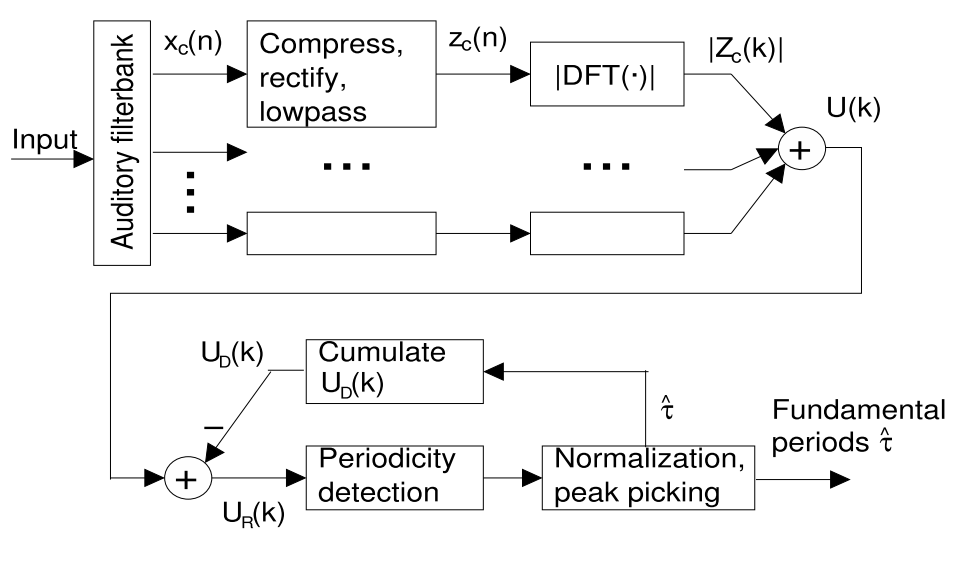
\includegraphics[scale=.25]{pitch_klapuri}
        \end{columns}
    \bigskip
    
    \begin{flushright}
        graph from \footfullcite{klapuri_perceptually_2005}
    \end{flushright}
	\end{frame}
    
    \section{summary}
        \begin{frame}{summary}{lecture content}
            \begin{itemize}
                \item   \textbf{polyphonic pitch detection}
                    \begin{itemize}
                        \item   highly challenging task with
                            \begin{itemize}
                                \item   unknown number of sources
                                \item   unknown harmonic structure
                                \item   spectral overlap of sources
                                \item   time-varying mixture
                            \end{itemize}
                    \end{itemize}
                \bigskip
                \item   \textbf{typical approaches}
                    \begin{itemize}
                        \item   iterative subtraction (detect one pitch, remove it, repeat analysis)
                        \item   multi-band processing
                    \end{itemize}
            \end{itemize}
            \inserticon{summary}
        \end{frame}
\end{document}
